%%%%%%%%%%%%%%%%%%%%%%%%%%%%%%%%%%%%%%%%%%%%%%%%%%%%%%%%%%%%%%%%%%%%%%%%%%%%%%%%%%%%%%%%%%%%%%%%%%%%%
% DOCUMENT CLASS
%%%%%%%%%%%%%%%%%%%%%%%%%%%%%%%%%%%%%%%%%%%%%%%%%%%%%%%%%%%%%%%%%%%%%%%%%%%%%%%%%%%%%%%%%%%%%%%%%%%%%%

% Single-spaced, two-column with PRL look and style (easy on the eyes)
\documentclass[aps,pre,twocolumn,superscriptaddress]{revtex4-1}
%\documentclass[aps,pre,twocolumn,superscriptaddress]{revtex4}

% Double-spaced, one-column style (for submission/review/editing)
%\documentclass[aps,preprint,prl,superscriptaddress,showpacs]{revtex4}

%%%%%%%%%%%%%%%%%%%%%%%%%%%%%%%%%%%%%%%%%%%%%%%%%%%%%%%%%%%%%%%%%%%%%%%%%%%%%%%%%%%%%%%%%%%%%%%%%%%%%%
% PREAMBLE
%%%%%%%%%%%%%%%%%%%%%%%%%%%%%%%%%%%%%%%%%%%%%%%%%%%%%%%%%%%%%%%%%%%%%%%%%%%%%%%%%%%%%%%%%%%%%%%%%%%%%%

\usepackage{palatino}
\usepackage{amsmath}
\usepackage{amssymb}
\usepackage{graphicx}
\usepackage{dcolumn}
\usepackage{boxedminipage}
\usepackage{verbatim}
\usepackage{booktabs}

\usepackage[colorlinks=true,citecolor=blue,linkcolor=blue]{hyperref}

% The figures are in a figures/ subdirectory.
\graphicspath{{../figures/}}

%\bibliographystyle{apsrevlong}
\bibliographystyle{apsrev}

% italicized boldface for math (e.g. vectors)
\newcommand{\bfv}[1]{{\mbox{\boldmath{$#1$}}}}
% non-italicized boldface for math (e.g. matrices)
\newcommand{\bfm}[1]{{\bf #1}}          

%\newcommand{\bfm}[1]{{\mbox{\boldmath{$#1$}}}}
%\newcommand{\bfm}[1]{{\bf #1}}
\newcommand{\expect}[1]{\left \langle #1 \right \rangle}                % <.> for denoting expectations over realizations of an experiment or thermal averages
\newcommand{\dhdl}{\frac{dH}{d\lambda}}
% vectors
\newcommand{\var}[1]{{\mathrm var}{(#1)}}
\newcommand{\x}{\bfv{x}}
\newcommand{\y}{\bfv{y}}
\newcommand{\f}{\bfv{f}}

\newcommand{\bfc}{\bfm{c}}
\newcommand{\hatf}{\hat{f}}

\newcommand{\bTheta}{\bfm{\Theta}}
\newcommand{\btheta}{\bfm{\theta}}
\newcommand{\bhatf}{\bfm{\hat{f}}}
\newcommand{\Cov}[1] {\mathrm{cov}\left( #1 \right)}
\newcommand{\Ept}[1] {{\mathrm E}\left[ #1 \right]}
\newcommand{\Eptk}[2] {{\mathrm E}_{#1}\left[ #2\right]}
\newcommand{\T}{\mathrm{T}}                                % T used in matrix transpose

\begin{document}



%\title{Benchmarking GAFF against Pure Liquid Properties in ThermoML}
%\title{Benchmarking Neat Liquid Simulations against the ThermoML Database}
\title{Benchmarking Simulations against the ThermoML Database: Neat Liquid Densities and Static Dielectrics}

 \author{Kyle A. Beauchamp}
 \affiliation{Memorial Sloan-Kettering Cancer Center, New York, NY, USA}

 \author{Julie M. Behr}
 \affiliation{Memorial Sloan-Kettering Cancer Center, New York, NY, USA}

\author{Patrick B. Grinaway }
 \affiliation{Memorial Sloan-Kettering Cancer Center, New York, NY, USA}

\author{Bas}
 \affiliation{Memorial Sloan-Kettering Cancer Center, New York, NY, USA}

 \author{Kenneth Kronlein}
 \affiliation{NIST}
 
 \author{Michael R. Shirts}
  \email{michael.shirts@virgina.edu}
 \affiliation{Department of Chemical Engineering, University of Virginia, Charlottesville, VA 22094-0471}

 \author{John D. Chodera}
 \email{jchodera@mskcc.org}
 \affiliation{Memorial Sloan-Kettering Cancer Center, New York, NY, USA}

 
\date{\today}
\maketitle


\section{Abstract}

Useful atomistic simulations require accurate depictions of solvent.  Simple experimental observables, such as density and static dielectric constants, offer straightforward targets for evaluating forcefield quality.  Here we examine the possibilty of benchmarking atomistic models against the NIST ThermoML database of physicochemical measurements, which curates thousands of density, dielectric, and other measurements.  We present a detailed benchmark of the GAFF forcefield against measurements extracted from ThermoML and discuss the extent of available data for neat liquids.  We show that empirical polarizability models correct systematic biases inherent in predicting dielectric constants with fixed-charged forcefields.  Combining our dataset with the Virtual Chemistry benchmark set provides an extensive benchmark suite for liquid properties.  

\section{Introduction}

Intro

\section{Results}

\subsection{Neat Liquid Measurements in ThermoML}

To assess the feasibility of benchmarking organic molecule forcefields against ThermoML, we performed a number of queries to summarize the data content of ThermoML.

\begin{tabular}{lrr}
\toprule
{} &  Mass Density &  Static Dielectric \\
\midrule
0.  Full                        &               308248 &                                     4170 \\
1.  Druglike elements           &                37944 &                                      847 \\
2.  $\le10$ heavy atoms, $\le100$ atoms &                27393 &                                      773 \\
3.  Temperature                 &                16529 &                                      609 \\
4.  Pressure                    &                 8160 &                                      399 \\
5.  Aggregate T, P              &                 3443 &                                      382 \\
\bottomrule
\end{tabular}


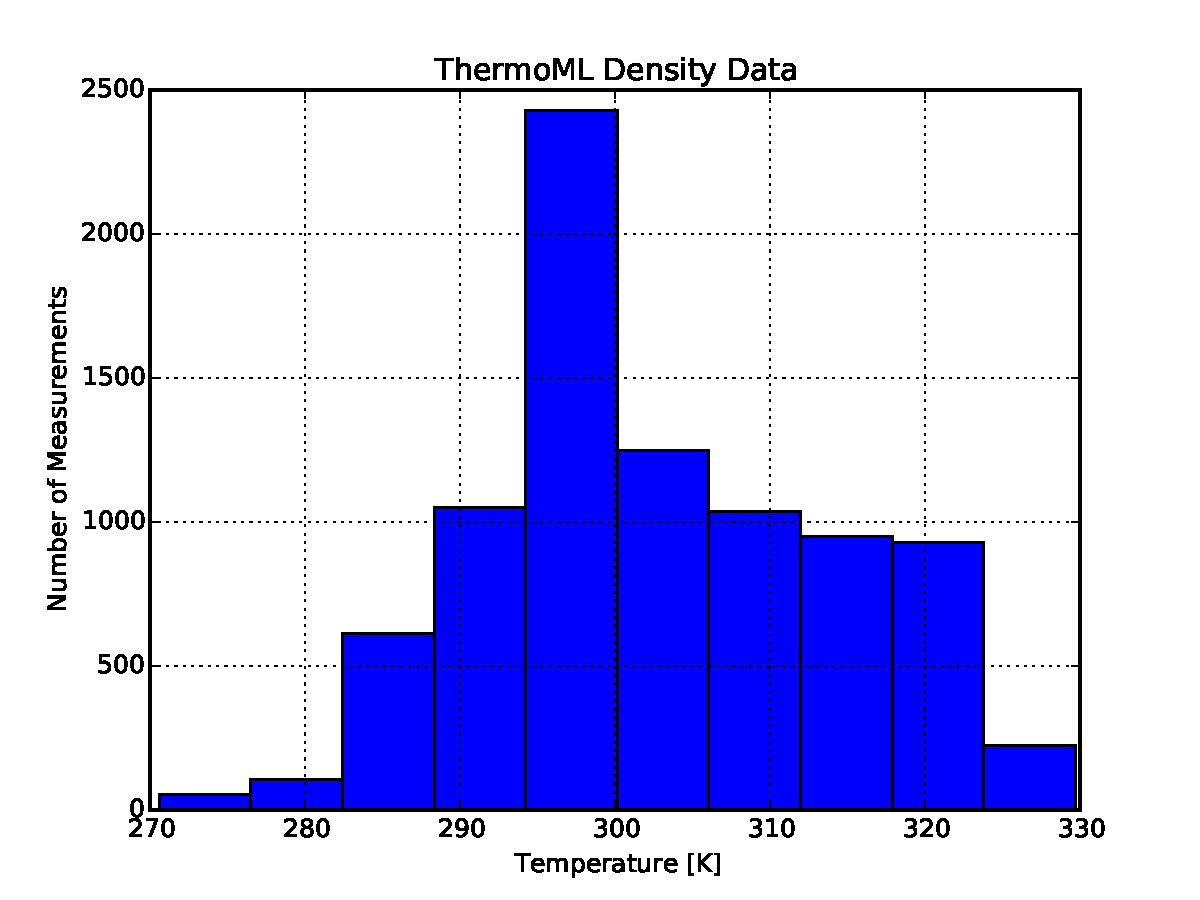
\includegraphics[width=\columnwidth]{./figures/thermoml_density_histogram.pdf}

\subsection{Benchmarking GAFF against ThermoML Measurements}

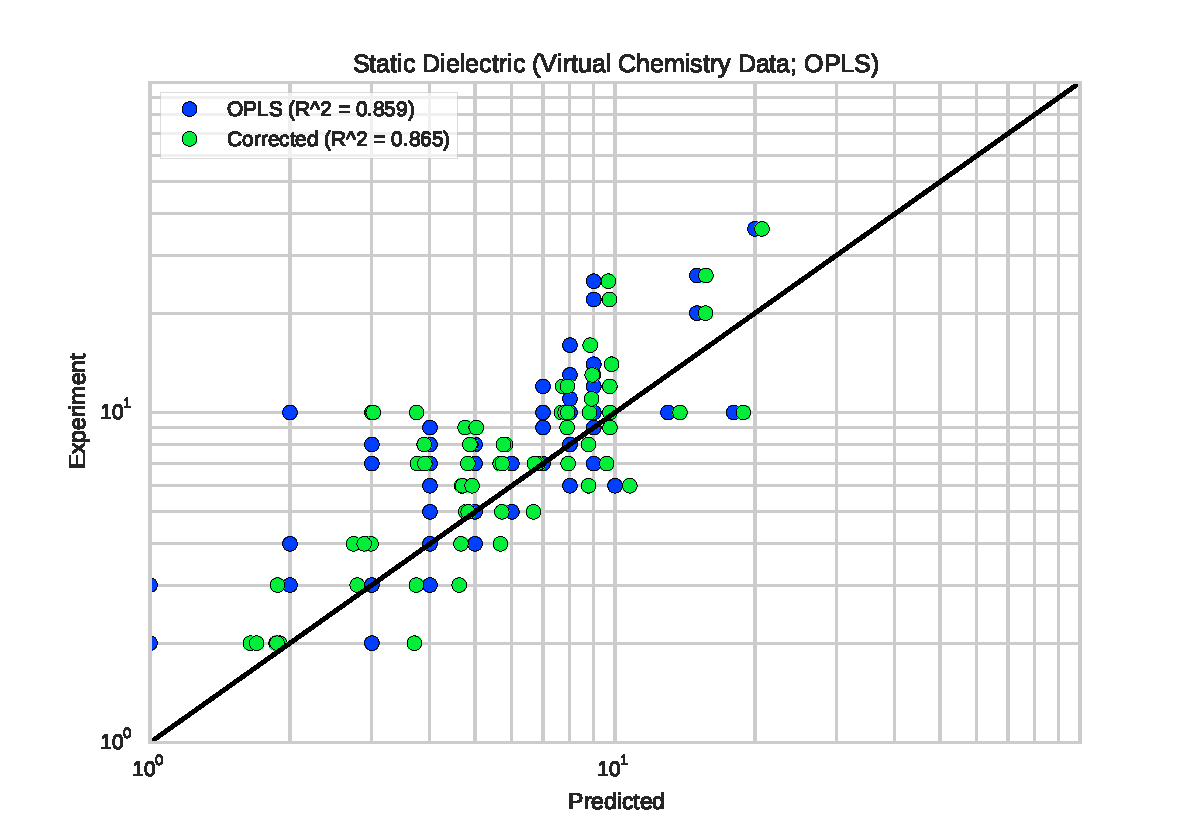
\includegraphics[width=\columnwidth]{./figures/dielectric_virtual_chemistry_opls.pdf}
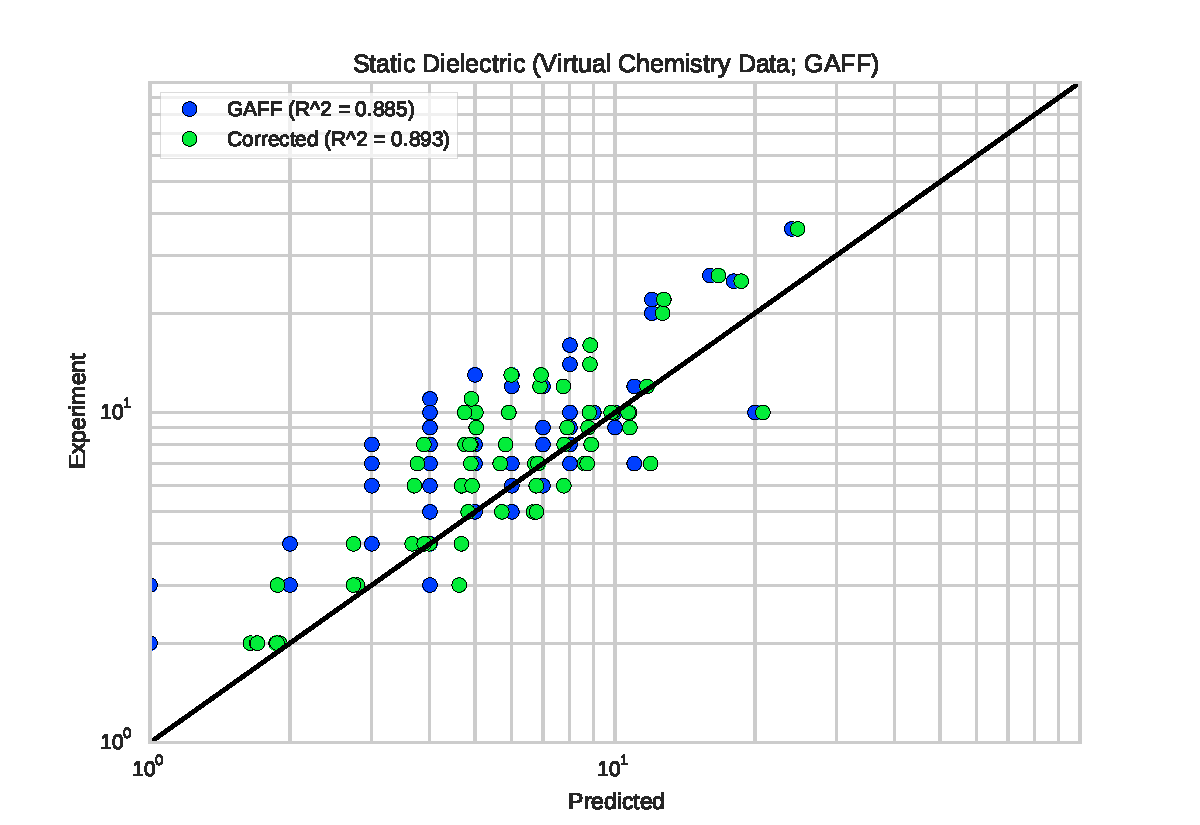
\includegraphics[width=\columnwidth]{./figures/dielectric_virtual_chemistry_gaff.pdf}
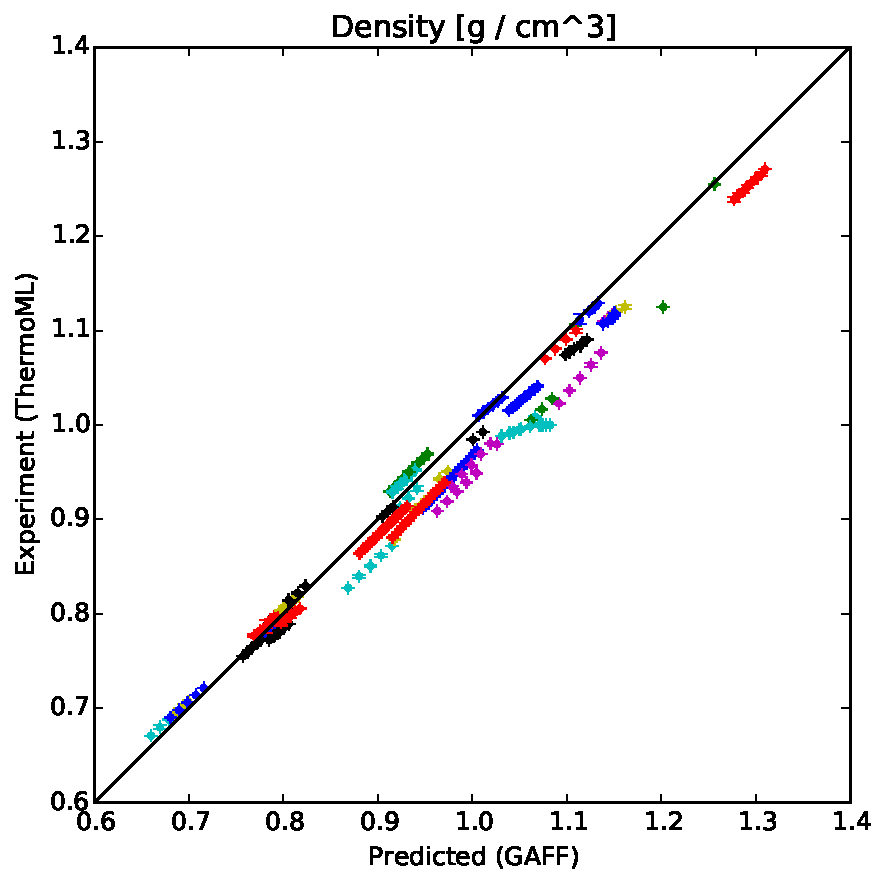
\includegraphics[width=\columnwidth]{./figures/densities_thermoml.pdf}
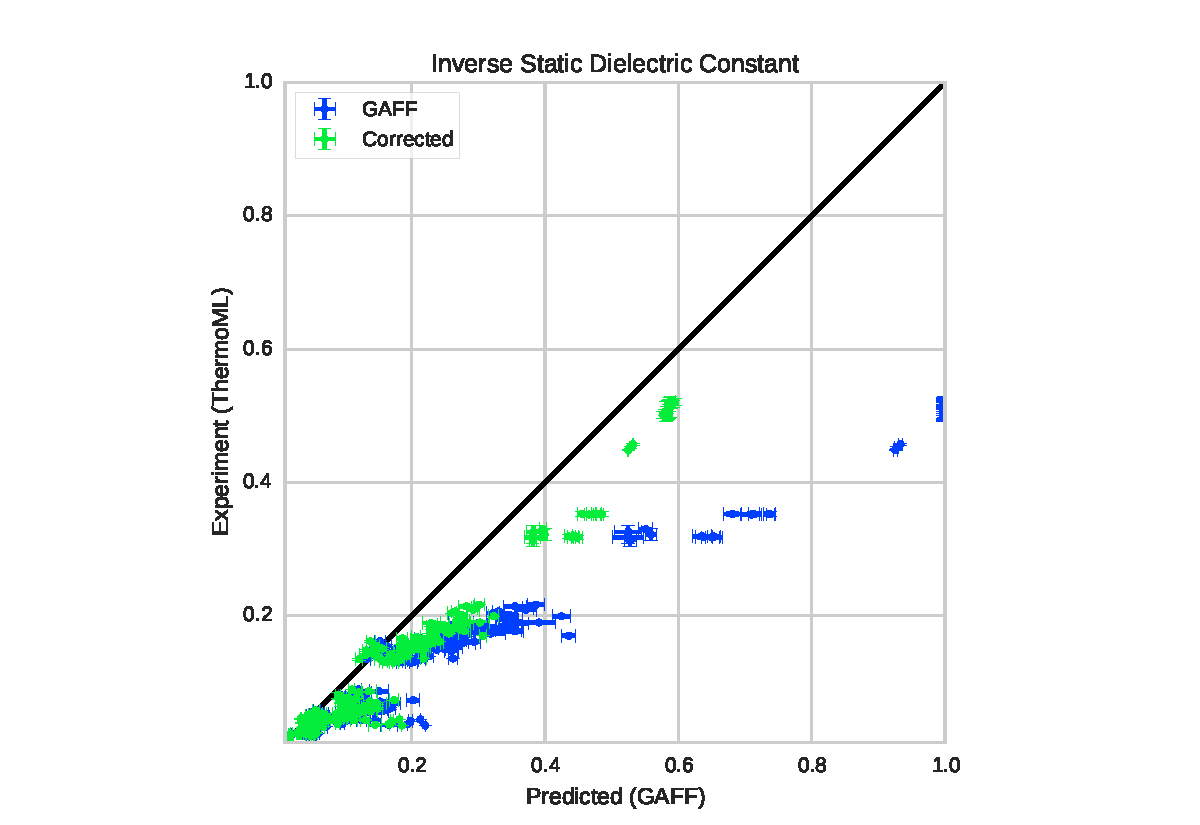
\includegraphics[width=\columnwidth]{./figures/dielectrics_thermoml.pdf}


\section{Discussion}

\subsection{Fitting Forcefields to Dielectric Constants}

Cite work by Chris Fennell on CCl4.  How to get a internally consistent model.  Static dielectric constant includes electronic polarization, need to subtract it out.  Cite TIP4PEW paper.  Could use frequency-dependent dielectric, but empirical polarizability models are highly accurate.  Cite LPW CCL4 paper.  Use idea of a molecular series CCL0 -> CCL1 ... CCL4 as example of internally inconcistent model when directly fitting dielectric constant.

\end{document}